\section{Results}
\label{sec:results}

\subsection{Text-prompted organ localization}
\label{sec:results:phase1}

Table~\ref{tab:overall} reports our final model (checkpoint v5, epoch 11) on the
TotalSegmentator v2.0.1 test split across 11 organ classes, with per-class
IoU-optimal thresholds. We reach a mean IoU of 0.653 and a mean Dice of 0.757
using no per-pixel labels at inference. The prompt alone selects the organ.

\begin{table}[t]
\centering
\caption{Our final model on the TotalSegmentator test split (11 organ classes,
2D per-slice metrics on organ-present slices). HD95 is in pixels on a
$224\times224$ grid.}
\label{tab:overall}
\begin{tabular}{lc}
\toprule
Metric & v5, epoch 11 (per-class tuned thresholds) \\
\midrule
mIoU              & \textbf{0.653} \\
Dice              & \textbf{0.757} \\
HD95 (px)         & 18.8 \\
Sensitivity       & 0.805 \\
Precision         & 0.749 \\
RVE               & 0.93 \\
NSD ($\tau=3$\,px) & 0.557 \\
\bottomrule
\end{tabular}
\end{table}

\paragraph{Ablation progression.}
Table~\ref{tab:progression} decomposes that number into the sequence of changes
that produced it. Each row adds one change to the row above. These are stages of
one method, not competing methods. We report the untrained row to show where our
pipeline begins, not as a comparison baseline; for that, see
\S\ref{sec:results:comparison}.

\begin{table}[t]
\centering
\caption{Ablation progression. Each row adds one change to the row above it.}
\label{tab:progression}
\begin{tabular}{llc}
\toprule
Version & Change & mIoU \\
\midrule
--         & Vanilla-gradient CAM, no fine-tuning (untrained starting point) & 0.003 \\
v0         & Grad-CAM + SigLIP fine-tuning                                   & 0.063 \\
v1         & \quad + patch-level contrastive loss                            & 0.307 \\
v3         & \quad + resume from v1                                          & 0.469 \\
v4         & \quad + resume from v3                                          & 0.574 \\
v4-tuned   & \quad + calibration fix (raw similarities, per-class IoU-optimal thresholds) & 0.633 \\
\textbf{v5-tuned} & \quad + one further 20-epoch resume from v4              & \textbf{0.653} \\
\bottomrule
\end{tabular}
\end{table}

Two steps deserve comment. First, our patch-level contrastive loss is the single
largest contributor, taking mIoU from 0.063 to 0.307. CLS-level contrastive
fine-tuning alone does not make patch similarity spatially meaningful. Second,
our calibration fix required \emph{no retraining} and added $+0.059$ mIoU while
halving HD95. Diagnostic analysis of the raw patch-text similarity distributions
showed us that per-image min--max normalization was destroying model-confidence
information, since it forces every slice to span the full dynamic range whether
or not the organ is present, and that class-conditional negative subtraction was
removing more foreground than background signal. Removing both, and sweeping
per-class IoU-optimal cutoffs on generated masks, recovered that 0.059 from the
same weights.

Our final resume run (v4-tuned $\to$ v5-tuned) added $+0.020$ mIoU overall but
concentrated its gains on the hardest classes: pancreas $+21\%$, kidney-right
$+15\%$, femur-right $+10\%$, while liver, lungs, heart and bladder had already
saturated at v4-tuned.

\paragraph{Per-class results.}
Table~\ref{tab:perclass} shows the per-class breakdown, which we consider the
more informative view: performance tracks organ size and contrast almost
monotonically. Large, morphologically distinct organs (lungs, liver, heart)
reach 0.79--0.83 IoU from text supervision alone. Pancreas, small and
low-contrast, reaches 0.29. Figure~\ref{fig:totalsegqual} shows the
corresponding masks.

\begin{table}[t]
\centering
\caption{Per-class IoU and Dice for our final model. $N$ is the number of
evaluated organ-present slices.}
\label{tab:perclass}
\begin{tabular}{lrrr}
\toprule
Organ & $N$ & IoU & Dice \\
\midrule
Lung right   & 535 & 0.828 & 0.897 \\
Liver        & 492 & 0.823 & 0.893 \\
Lung left    & 545 & 0.798 & 0.875 \\
Heart        & 480 & 0.787 & 0.866 \\
Bladder      & 265 & 0.698 & 0.796 \\
Spleen       & 464 & 0.644 & 0.768 \\
Femur left   & 260 & 0.587 & 0.722 \\
Femur right  & 262 & 0.565 & 0.706 \\
Kidney left  & 401 & 0.491 & 0.627 \\
Kidney right & 403 & 0.453 & 0.595 \\
Pancreas     & 395 & 0.290 & 0.419 \\
\bottomrule
\end{tabular}
\end{table}

\begin{figure}[t]
\centering
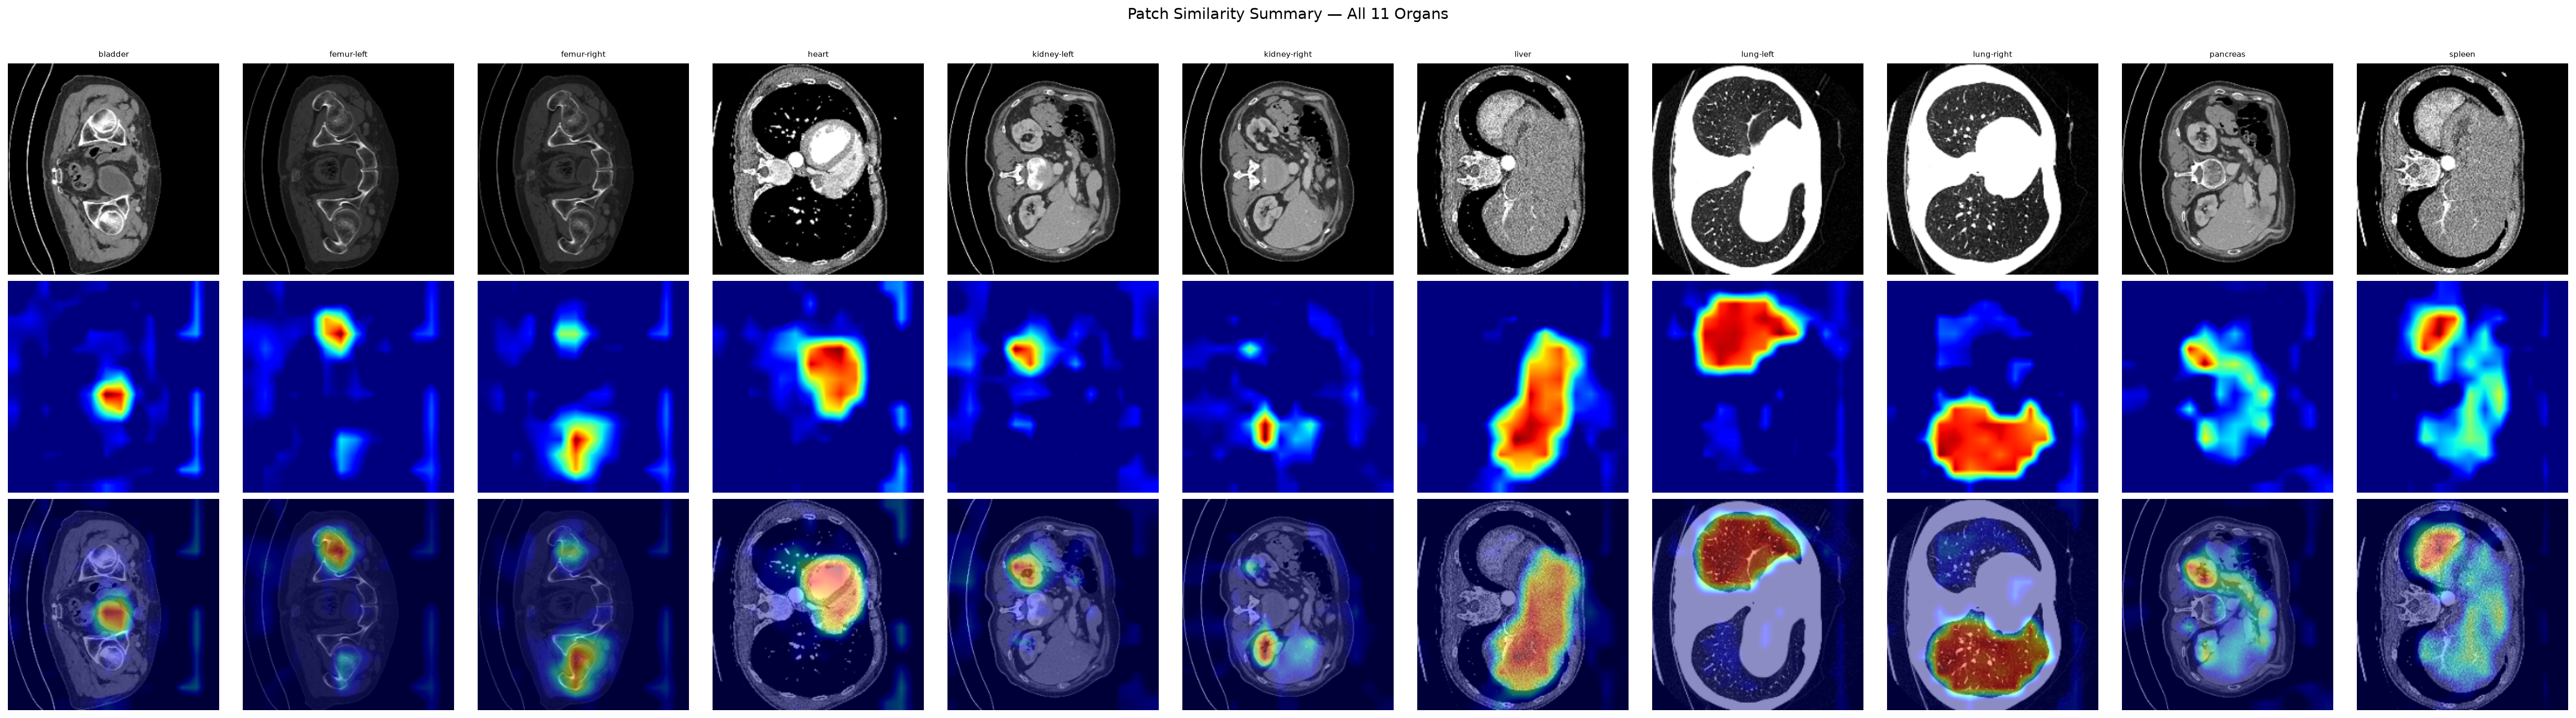
\includegraphics[width=\textwidth]{totalseg/totalseg_summary.png}
\caption{Generated masks on the TotalSegmentator test split, one column per
organ class. Large, high-contrast structures (lungs, liver, heart) are recovered
with clean boundaries from the prompt alone; the degradation on smaller,
lower-contrast structures (pancreas, kidneys) is visible as boundary spill
rather than as gross mislocalization, which is consistent with the per-class
ordering in Table~\ref{tab:perclass} and with the $14\times14$ patch grid
bounding attainable boundary precision.}
\label{fig:totalsegqual}
\end{figure}

\subsection{What the prompt actually contributes}
\label{sec:results:ablation}

A text-conditioned localizer invites an obvious objection: the text may be a
passenger, with the visual encoder doing all the work and the prompt serving
only as a class index. To test this we re-evaluated the fine-tuned v4 model with
five prompt formulations, changing only the text embedding and retraining
nothing (Table~\ref{tab:captions}).

\begin{table}[t]
\centering
\caption{Caption ablation. Text embeddings are the only variable; no retraining.
L5 is L4 with LEFT$\leftrightarrow$RIGHT and top$\leftrightarrow$bottom swapped.
We mark L4 because it is the formulation used during training, \emph{not}
because it wins. L2 and L4 are indistinguishable and in fact split the two
metrics: L2 is ahead on mIoU by 0.0006 (0.6273 vs.\ 0.6267) and L4 is ahead on
Dice by 0.0006 (0.7441 vs.\ 0.7435).}
\label{tab:captions}
\begin{tabular}{llrr}
\toprule
Level & Prompt formulation & mIoU & Dice \\
\midrule
L1 & Class name only                                  & 0.607 & 0.728 \\
L2 & Generic clinical caption                         & 0.627 & 0.743 \\
L3 & Position only (organ name removed)               & 0.561 & 0.684 \\
L4$^{*}$ & Full anatomical description (used in training) & 0.627 & 0.744 \\
L5 & Adversarial (L4 with position words swapped)     & 0.458 & 0.583 \\
\bottomrule
\end{tabular}
\end{table}

\begin{figure}[t]
\centering
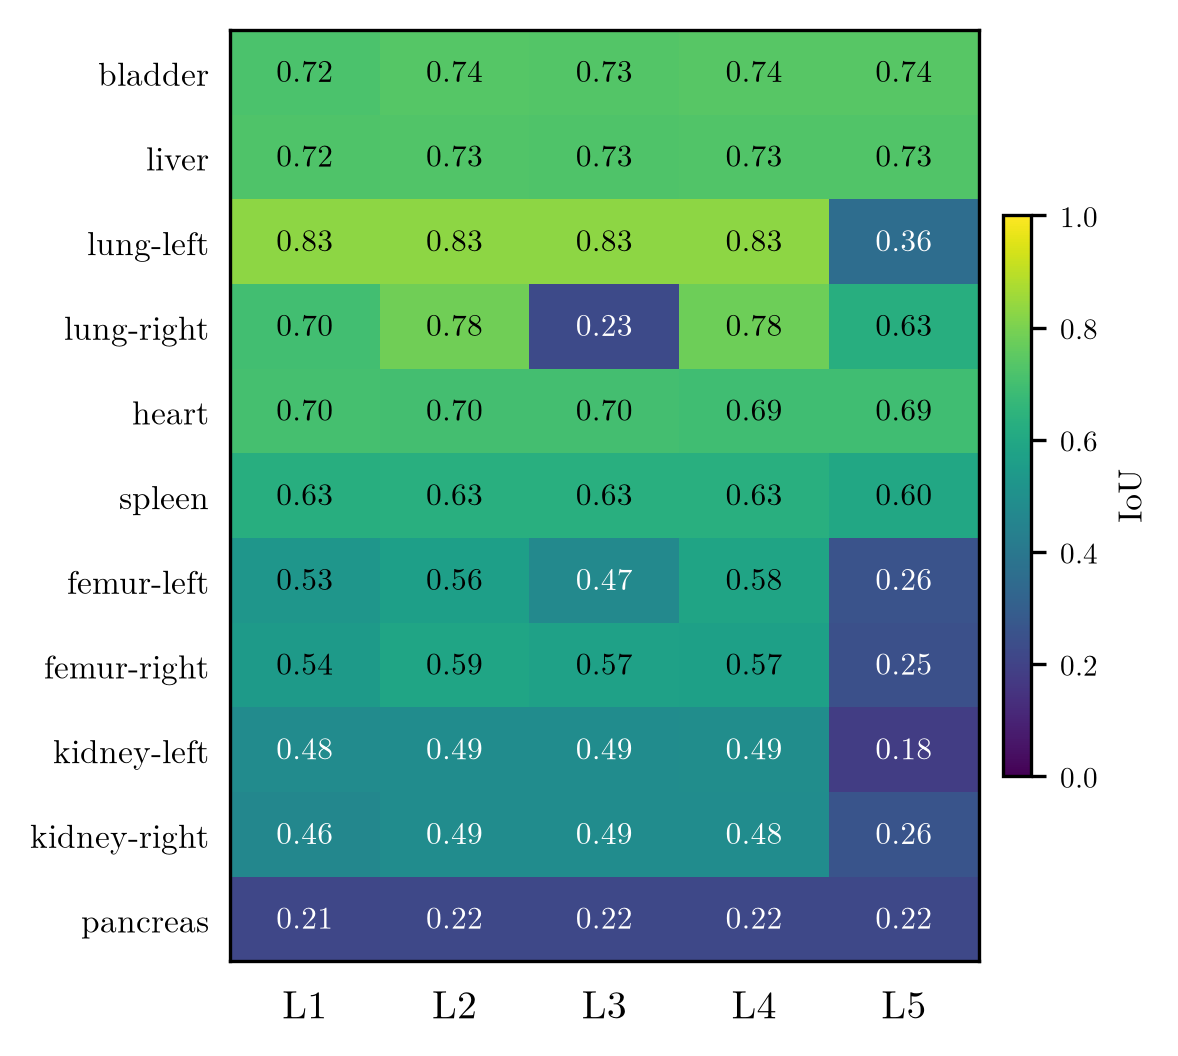
\includegraphics[width=0.74\textwidth]{caption_ablation.png}
\caption{Per-class IoU across the five prompt formulations, with bilateral pairs
placed adjacently and groups ordered easy to hard, so each pair can be read
against itself. Three features are visible directly. Classes whose identity
rests on a laterality word collapse in the L5 column (kidney-left
$0.49\to0.18$, femurs $\approx 0.58\to0.26$, lung-left $0.83\to0.36$) while
uniquely-positioned classes are untouched by the same transformation (liver,
heart, bladder all unchanged to two decimals). The exception is instructive:
\org{lung-right} falls only $0.78\to0.63$, because its prompt asserts a
three-lobe morphology that survives a laterality swap, which is the mechanism of
finding 3a. The isolated dark cell at \org{lung-right}/L3 is the accidental
two-word prompt error discussed in the text, not a property of the L3 level, as
\org{lung-left} holds 0.83 in the same column. Pancreas is flat across the
entire row including L1, the clearest single statement that it is data-limited
rather than prompt-limited.}
\label{fig:captionheat}
\end{figure}

Four findings follow, and Figure~\ref{fig:captionheat} shows the per-class
structure behind them.

\textbf{(1) Class names carry most of the signal, and elaboration adds almost
nothing.} L1 reaches 96.9\% of L4's mIoU. Fine-tuning made the
organ-name-to-region mapping strong enough that a single word recovers nearly
everything a multi-sentence anatomical description provides. Anatomical detail
does not buy the remaining 3\% either. A one-line generic clinical caption (L2)
matches the full description (L4) to within 0.0006 on both metrics, and the two
split them: L2 is ahead on mIoU, L4 on Dice. We take that as a cleaner statement
of equivalence than either ordering alone would be. Whatever L1 is missing is
supplied by having \emph{any} sentence context at all, not by the anatomy
written into it.

\textbf{(2) Position language refines rather than substitutes.} L3, which keeps
position cues but removes organ identity, scores \emph{below} L1 (0.561 vs.\
0.607). The model needs to know what to look for before where becomes useful.

\textbf{(3) The text is not a passenger.} Under L5, classes that depend on
left/right disambiguation collapse (kidney-left $-63\%$, lung-left $-57\%$,
femurs $-56\%$) while organs with unique positions are unaffected (liver,
spleen, heart, bladder). The model demonstrably uses the positional content of
the prompt, and corrupting it degrades exactly the classes for which it matters.

\textbf{(3a) Adversarial robustness scales with position-invariant anatomical
content.} The two lungs receive the same L5 transformation and respond very
differently: lung-left falls $0.83\to0.36$ ($-57\%$), lung-right only
$0.78\to0.63$ ($-19\%$). The prompts explain the asymmetry. Lung-left's
distinguishing clause, \emph{``slightly smaller than the right due to the heart
pushing into the left hemithorax''}, inverts cleanly under the swap and ends up
describing the other lung, leaving nothing pointing at the correct organ.
Lung-right's prompt contains a clause the swap cannot corrupt: \emph{``Three
lobes are present, divided by fissures visible as thin lines.''} The right lung
genuinely has three lobes and the left has two, so that sentence still points at
the right lung however the position words are flipped. We regard this as
actionable rather than incidental: including morphological cues that are
invariant under position swaps (lobe count, characteristic shape) hardens a
bilateral class against precisely the failure mode L5 probes.

\textbf{(4) Pancreas is data-limited, not prompt-limited.} Pancreas IoU stays at
0.21--0.22 across \emph{every} level, including L1 (the bare word ``pancreas'')
and L4. Prompt engineering will not fix pancreas. The ceiling is inherent to our
approach for small, low-contrast structures.

\paragraph{An unintended natural experiment.}
We auto-generated the L3 prompts, and the one for \org{lung-right} came out
wrong in both of its content words. It read \emph{``The left lung occupies the
left half of the image''} where our L4 convention requires \emph{``The right
lung \ldots{} the left half.''} The organ name is wrong \emph{and} the position
is wrong, and the two errors are mutually consistent: the resulting sentence is
a valid description of the \emph{left} lung. The model did not become confused
or degrade gracefully. It followed the prompt and segmented the left lung. IoU
on \org{lung-right} at L3 fell to 0.23, while \org{lung-left} at L3 held at
0.829, essentially identical to its 0.828 at L4, confirming the L3 \emph{level}
is not itself harmful for lungs and isolating the cause to the two wrong words.

A two-word error in one of eleven prompts therefore cost 55 IoU points on the
affected class. More importantly, it shows the failure is \emph{directional}
rather than degradative: a wrong-but-internally-coherent prompt yields a
confident segmentation of the wrong structure. For clinical deployment we regard
that as a considerably more dangerous failure mode than low confidence, because
nothing in the output signals that anything went wrong.

\subsection{Comparison to supervised and weakly-supervised references}
\label{sec:results:comparison}

\paragraph{Fully-supervised ceiling.}
Table~\ref{tab:fullysup} places our per-class Dice against TotalSegmentator
\cite{wasserthal2023totalsegmentator}, a fully-supervised 3D nnU-Net
\cite{isensee2021nnunet} trained on the same dataset with dense per-voxel
labels.

\begin{table}[t]
\centering
\caption{Against the fully-supervised reference. \textbf{The two columns are not
the same metric and must not be subtracted}; see the caveat below.
$\dagger$~TotalSegmentator v1 segments the heart as separate chambers; range
spans myocardium (0.937) to left ventricle (0.955). $\ddagger$~Lungs are
segmented per-lobe; left $=$ upper/lower (0.971/0.985), right $=$
upper/middle/lower (0.944/0.975/0.988).}
\label{tab:fullysup}
\begin{tabular}{lrr}
\toprule
Organ & OrganPrompt Dice (2D, weakly sup.) & TotalSegmentator Dice (3D, fully sup.) \\
\midrule
Liver        & 0.893 & 0.965 \\
Spleen       & 0.768 & 0.983 \\
Kidney left  & 0.627 & 0.953 \\
Kidney right & 0.595 & 0.939 \\
Pancreas     & 0.419 & 0.887 \\
Bladder      & 0.796 & 0.934 \\
Femur left   & 0.722 & 0.914 \\
Femur right  & 0.706 & 0.942 \\
Heart        & 0.866 & 0.937--0.955$^\dagger$ \\
Lung left    & 0.875 & 0.971/0.985$^\ddagger$ \\
Lung right   & 0.897 & 0.944--0.988$^\ddagger$ \\
\bottomrule
\end{tabular}
\end{table}

\textbf{Metric caveat.} We report 2D per-slice Dice on organ-present axial
slices; TotalSegmentator reports 3D volumetric Dice over whole volumes. 2D slice
Dice on organ-present slices is systematically \emph{more forgiving}, because no
empty or partial-boundary slices drag the average down. The true
supervised-to-weakly-supervised gap is therefore \emph{wider} than the raw
column difference suggests, and we recommend reading the second column as an
approximate upper bound achievable \emph{with} full pixel supervision, not a
like-for-like benchmark.

With that caveat applied, the pattern is still informative. On large,
high-contrast organs we reach 0.87--0.90 slice Dice with no pixel labels, and
the gap widens exactly where weak supervision is expected to struggle: pancreas
0.42 vs.\ 0.89, kidneys 0.60--0.63 vs.\ 0.94--0.95.

\paragraph{Weakly-supervised methods, stratified by supervision strength.}
``Weakly supervised'' spans a wide range of annotation cost, and that range
drives the comparison. Point- and scribble-supervised methods receive per-image
\emph{spatial} information that we never see: a scribble already answers
``where,'' which is the entire problem we solve from text alone. We include them
in Table~\ref{tab:weaksup} for context and note explicitly that they are not
like-for-like.

\begin{table}[t]
\centering
\small
\caption{Published weakly-supervised methods, ordered by supervision strength.
Entries reporting relative gains cannot be placed on the same axis as absolute
Dice, and no row here shares both a dataset and a metric with our work.}
\label{tab:weaksup}
\begin{tabularx}{\textwidth}{@{}l l X X@{}}
\toprule
Method & Supervision & Task / dataset & Reported Dice \\
\midrule
\textbf{OrganPrompt (this work)} & \textbf{Image-level text} & 11 organs, TotalSegmentator (2D) & \textbf{0.42--0.90} (mean 0.742) \\
MedCLIP-SAMv2, zero-shot \cite{koleilat2025medclipsamv2} & Text, no masks & BUSI, brain MRI, COVID-QU-Ex, lung CT & 78.21 mean DSC \\
MedCLIP-SAMv2, weakly sup.\ \cite{koleilat2025medclipsamv2} & Text $+$ pseudo-labels & same four tasks & 82.11 mean DSC \\
PET-CT lesion CAM \cite{fruh2021petct} & Image-level & Tumor lesions, PET-CT & 0.47 median (vs.\ 0.72 fully sup.) \\
Probabilistic-aware \cite{jiang2024probabilistic} & Point & BTCV (CT), CHAOS (MRI) & $+18.1\%/+10.2\%$ over prior point sup. \\
Probabilistic-aware \cite{jiang2024probabilistic} & Scribble & BTCV (CT), CHAOS (MRI) & $+58.4\%/+17.6\%$ over prior scribble sup. \\
\bottomrule
\end{tabularx}
\end{table}

Three caveats apply before comparing any two rows. The datasets differ, since
BTCV, AMOS and WORD are the usual multi-organ weak-supervision benchmarks rather
than TotalSegmentator. The metrics differ, both in the 2D/3D sense above and
because MedCLIP-SAMv2 reports DSC on a 0--100 scale over a different organ set
entirely. And two entries report relative gains, because that is what the source
publishes. We deliberately do not compute a ``gap'' between any two rows of this
table.

Within the image-level tier, which is the only strictly comparable one, our
per-organ range (0.42--0.90) sits above the image-level PET-CT CAM result (0.47
median), on a different task. Our closest methodological relative is
MedCLIP-SAMv2 \cite{koleilat2025medclipsamv2}, which shares the BiomedCLIP
backbone and the text-driven premise but pairs it with SAM
\cite{kirillov2023sam} for mask refinement instead of reading patch similarity
directly. We regard that difference as the point of comparison rather than the
scores: delegating mask formation to a second model makes the pipeline stronger,
and also makes it impossible to attribute a failure to the prompt, which is what
our caption ablation in \S\ref{sec:results:ablation} depends on being able to
do.

An earlier version of this comparison included a representative
scribble-supervised multi-organ CT result. We removed it. We could not trace the
figures to a specific publication, and an untraceable row is worse than an
absent one in a table whose whole purpose is to calibrate expectations. Our
honest summary of the point- and scribble-supervised tier is therefore
qualitative: those methods receive a per-image spatial hint that answers
``where,'' report 3D volumetric Dice on different organ sets, and we do not
measure ourselves against them here. What Table~\ref{tab:fullysup} already
establishes is the shape that matters: our deficit concentrates in small,
low-contrast structures (pancreas, kidneys) and nearly closes for large,
high-contrast ones.

\subsection{Bone-metastasis proximity index}
\label{sec:results:index}

The second half of our work applies the same frozen patch-similarity model to a
different question: given a vertebral metastasis, which organ is it closest to
invading? Figure~\ref{fig:organgrid} shows all 11 organ maps on a thoracic
lesion slice from Spine-Mets-CT-SEG \cite{pieper2024spinemets}, a dataset and CT
protocol our model was never trained on.

\begin{figure}[t]
\centering
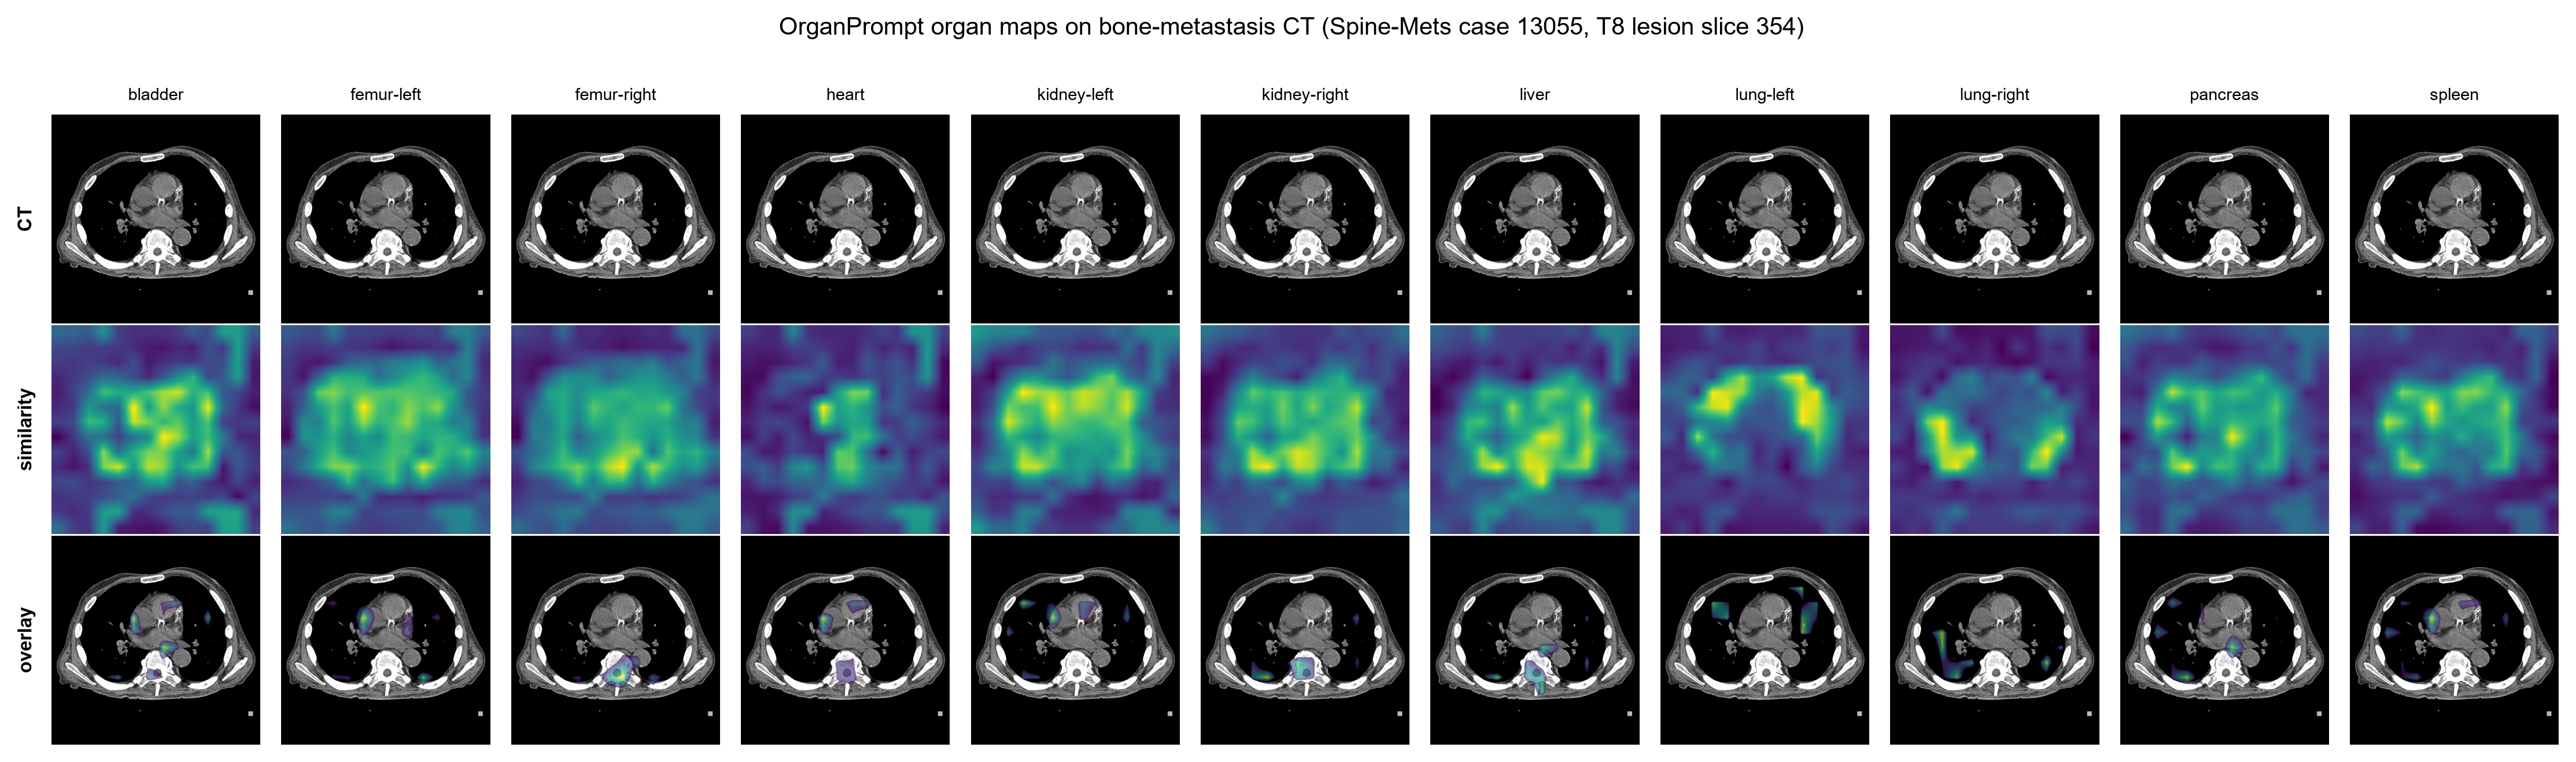
\includegraphics[width=\textwidth]{fig4_spine_organ_grid.png}
\caption{All 11 organ maps on a single Spine-Mets thoracic lesion slice (case
13055, T8 lesion). Rows: CT, raw patch-text similarity, overlay. We highlight
the top 2\% of each slice's own similarity distribution rather than an absolute
cutoff, because raw similarity is routinely negative across an entire slice and
organs win relatively rather than absolutely, so an absolute-zero threshold
renders most panels blank. We show the T8 \emph{lesion} slice rather than the
patient's peak-tumor slice, which sits at the pelvis where heart, lungs, liver
and spleen are out of frame; that slice would display noise in those columns and
wrongly imply the model hallucinates organs that are in fact absent.}
\label{fig:organgrid}
\end{figure}

Across the 46 labelled patients our index has mean 0.139 and median 0.083, with
9 patients below 0.01 and a smaller cluster of clearly-involved cases in the
0.25--0.50 range (maximum 0.500). Figure~\ref{fig:indexdist} shows the
distribution and Figure~\ref{fig:lesionoverlays} shows what low, mid and high
scores look like. We read the right-skewed shape as the expected mix of indolent
and locally aggressive metastases, not a calibration artifact.

\begin{figure}[t]
\centering
\begin{subfigure}{0.48\textwidth}
  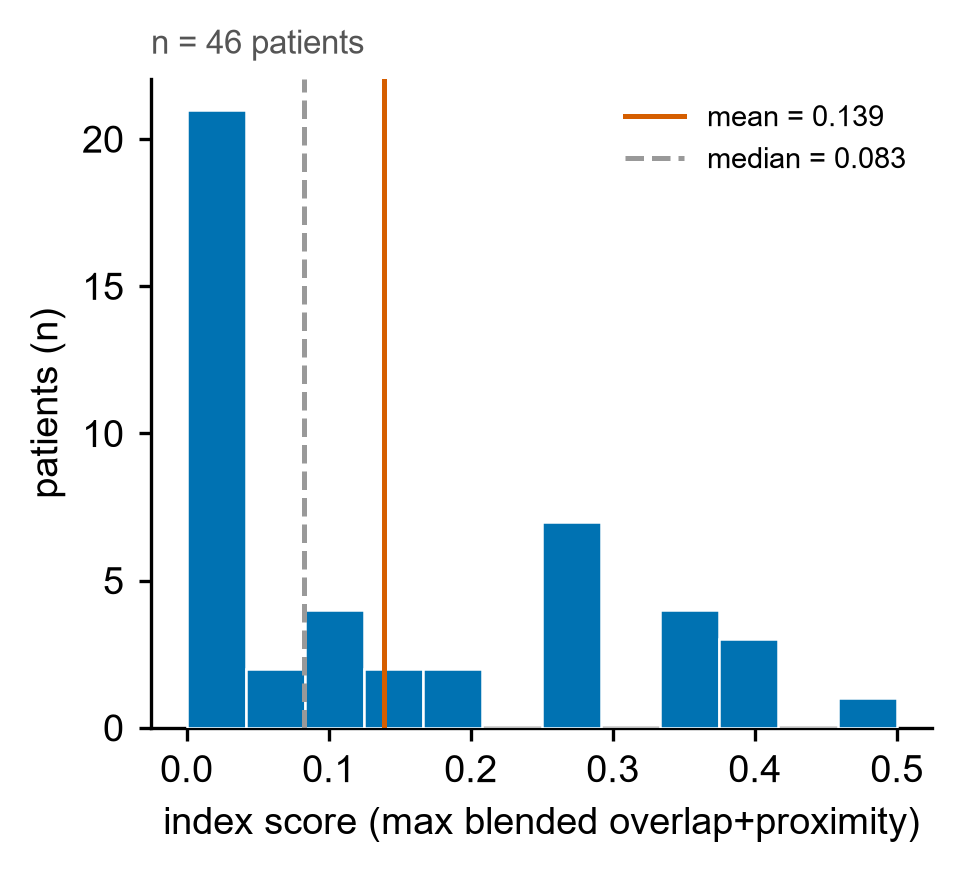
\includegraphics[width=\textwidth]{fig2_index_dist.png}
  \caption{}\label{fig:indexdist}
\end{subfigure}\hfill
\begin{subfigure}{0.48\textwidth}
  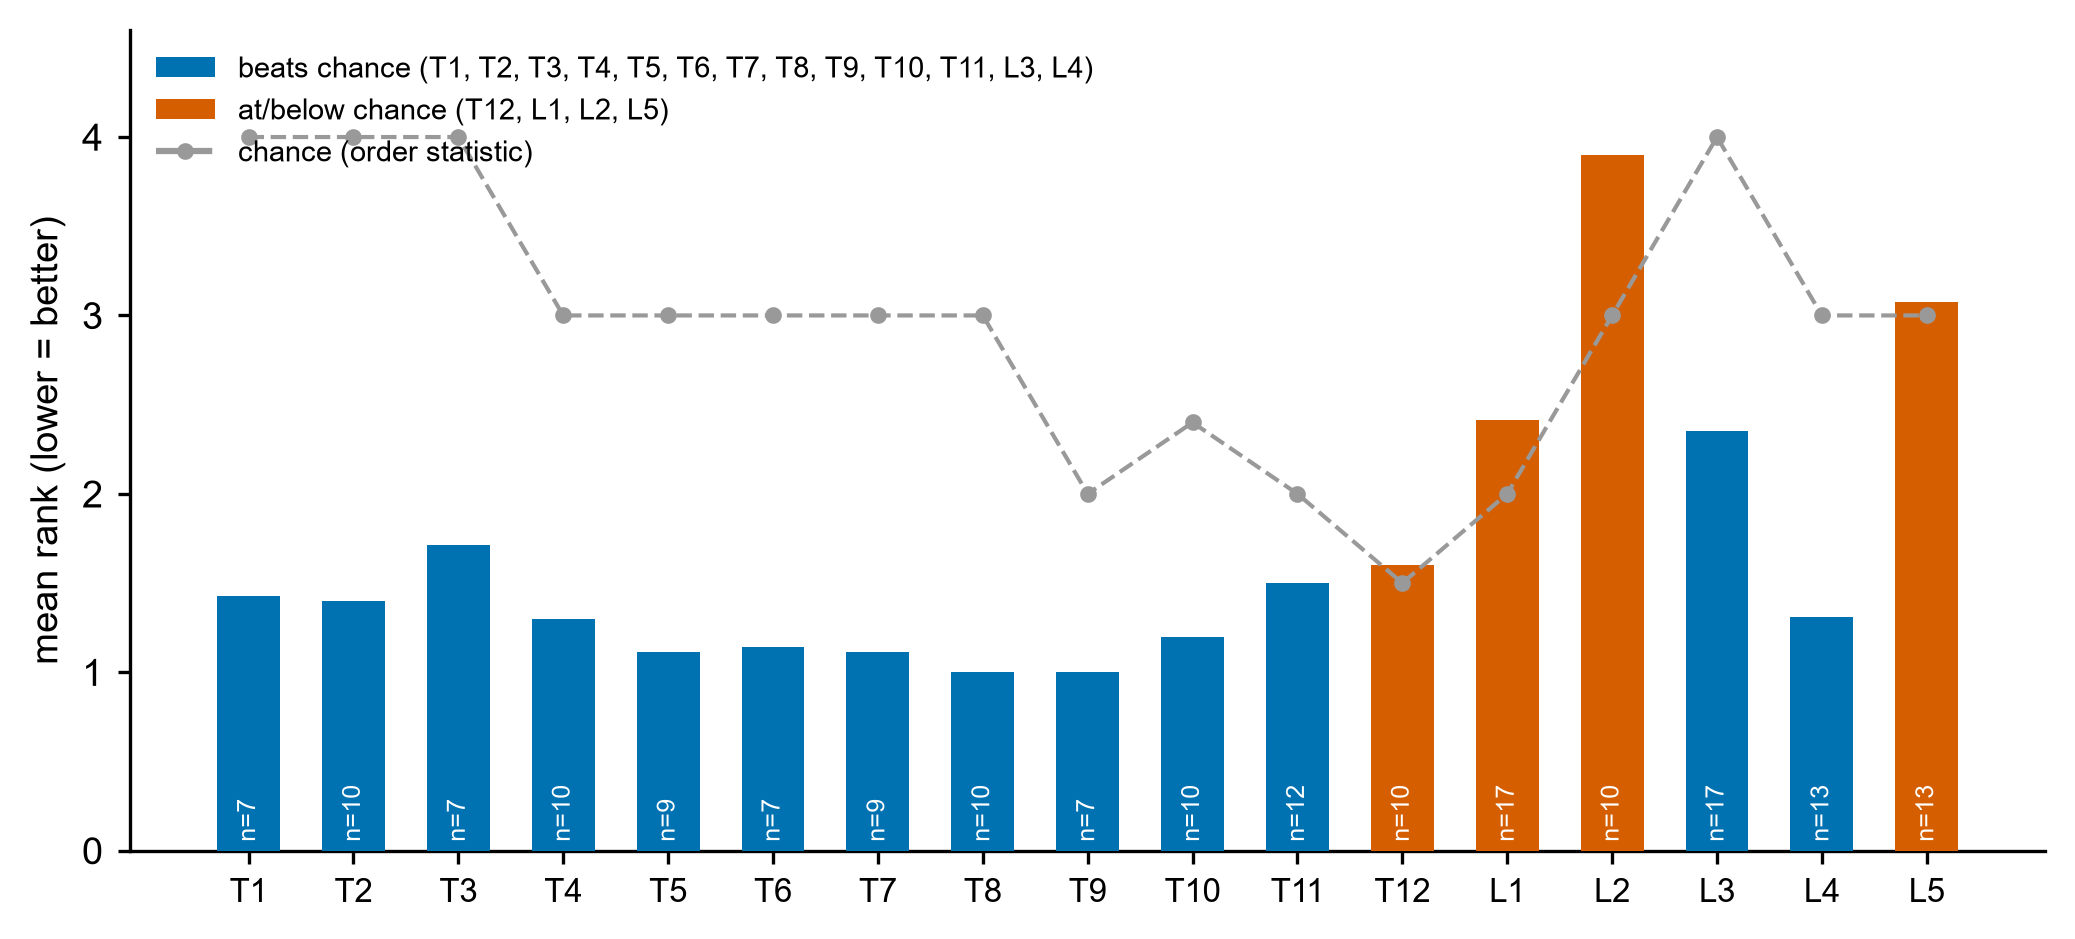
\includegraphics[width=\textwidth]{fig1_per_level.png}
  \caption{}\label{fig:perlevel}
\end{subfigure}
\caption{(\subref{fig:indexdist}) Per-patient index score across $n=46$
labelled patients, on the unleaked calibration. (\subref{fig:perlevel})
Per-vertebral-level mean rank of the correct organ(s) against that level's
chance mean rank (grey dashed). We derive bar colour from each level's own
observed-vs-chance comparison. $n$ per level is annotated inside each bar.}
\end{figure}

\begin{figure}[t]
\centering
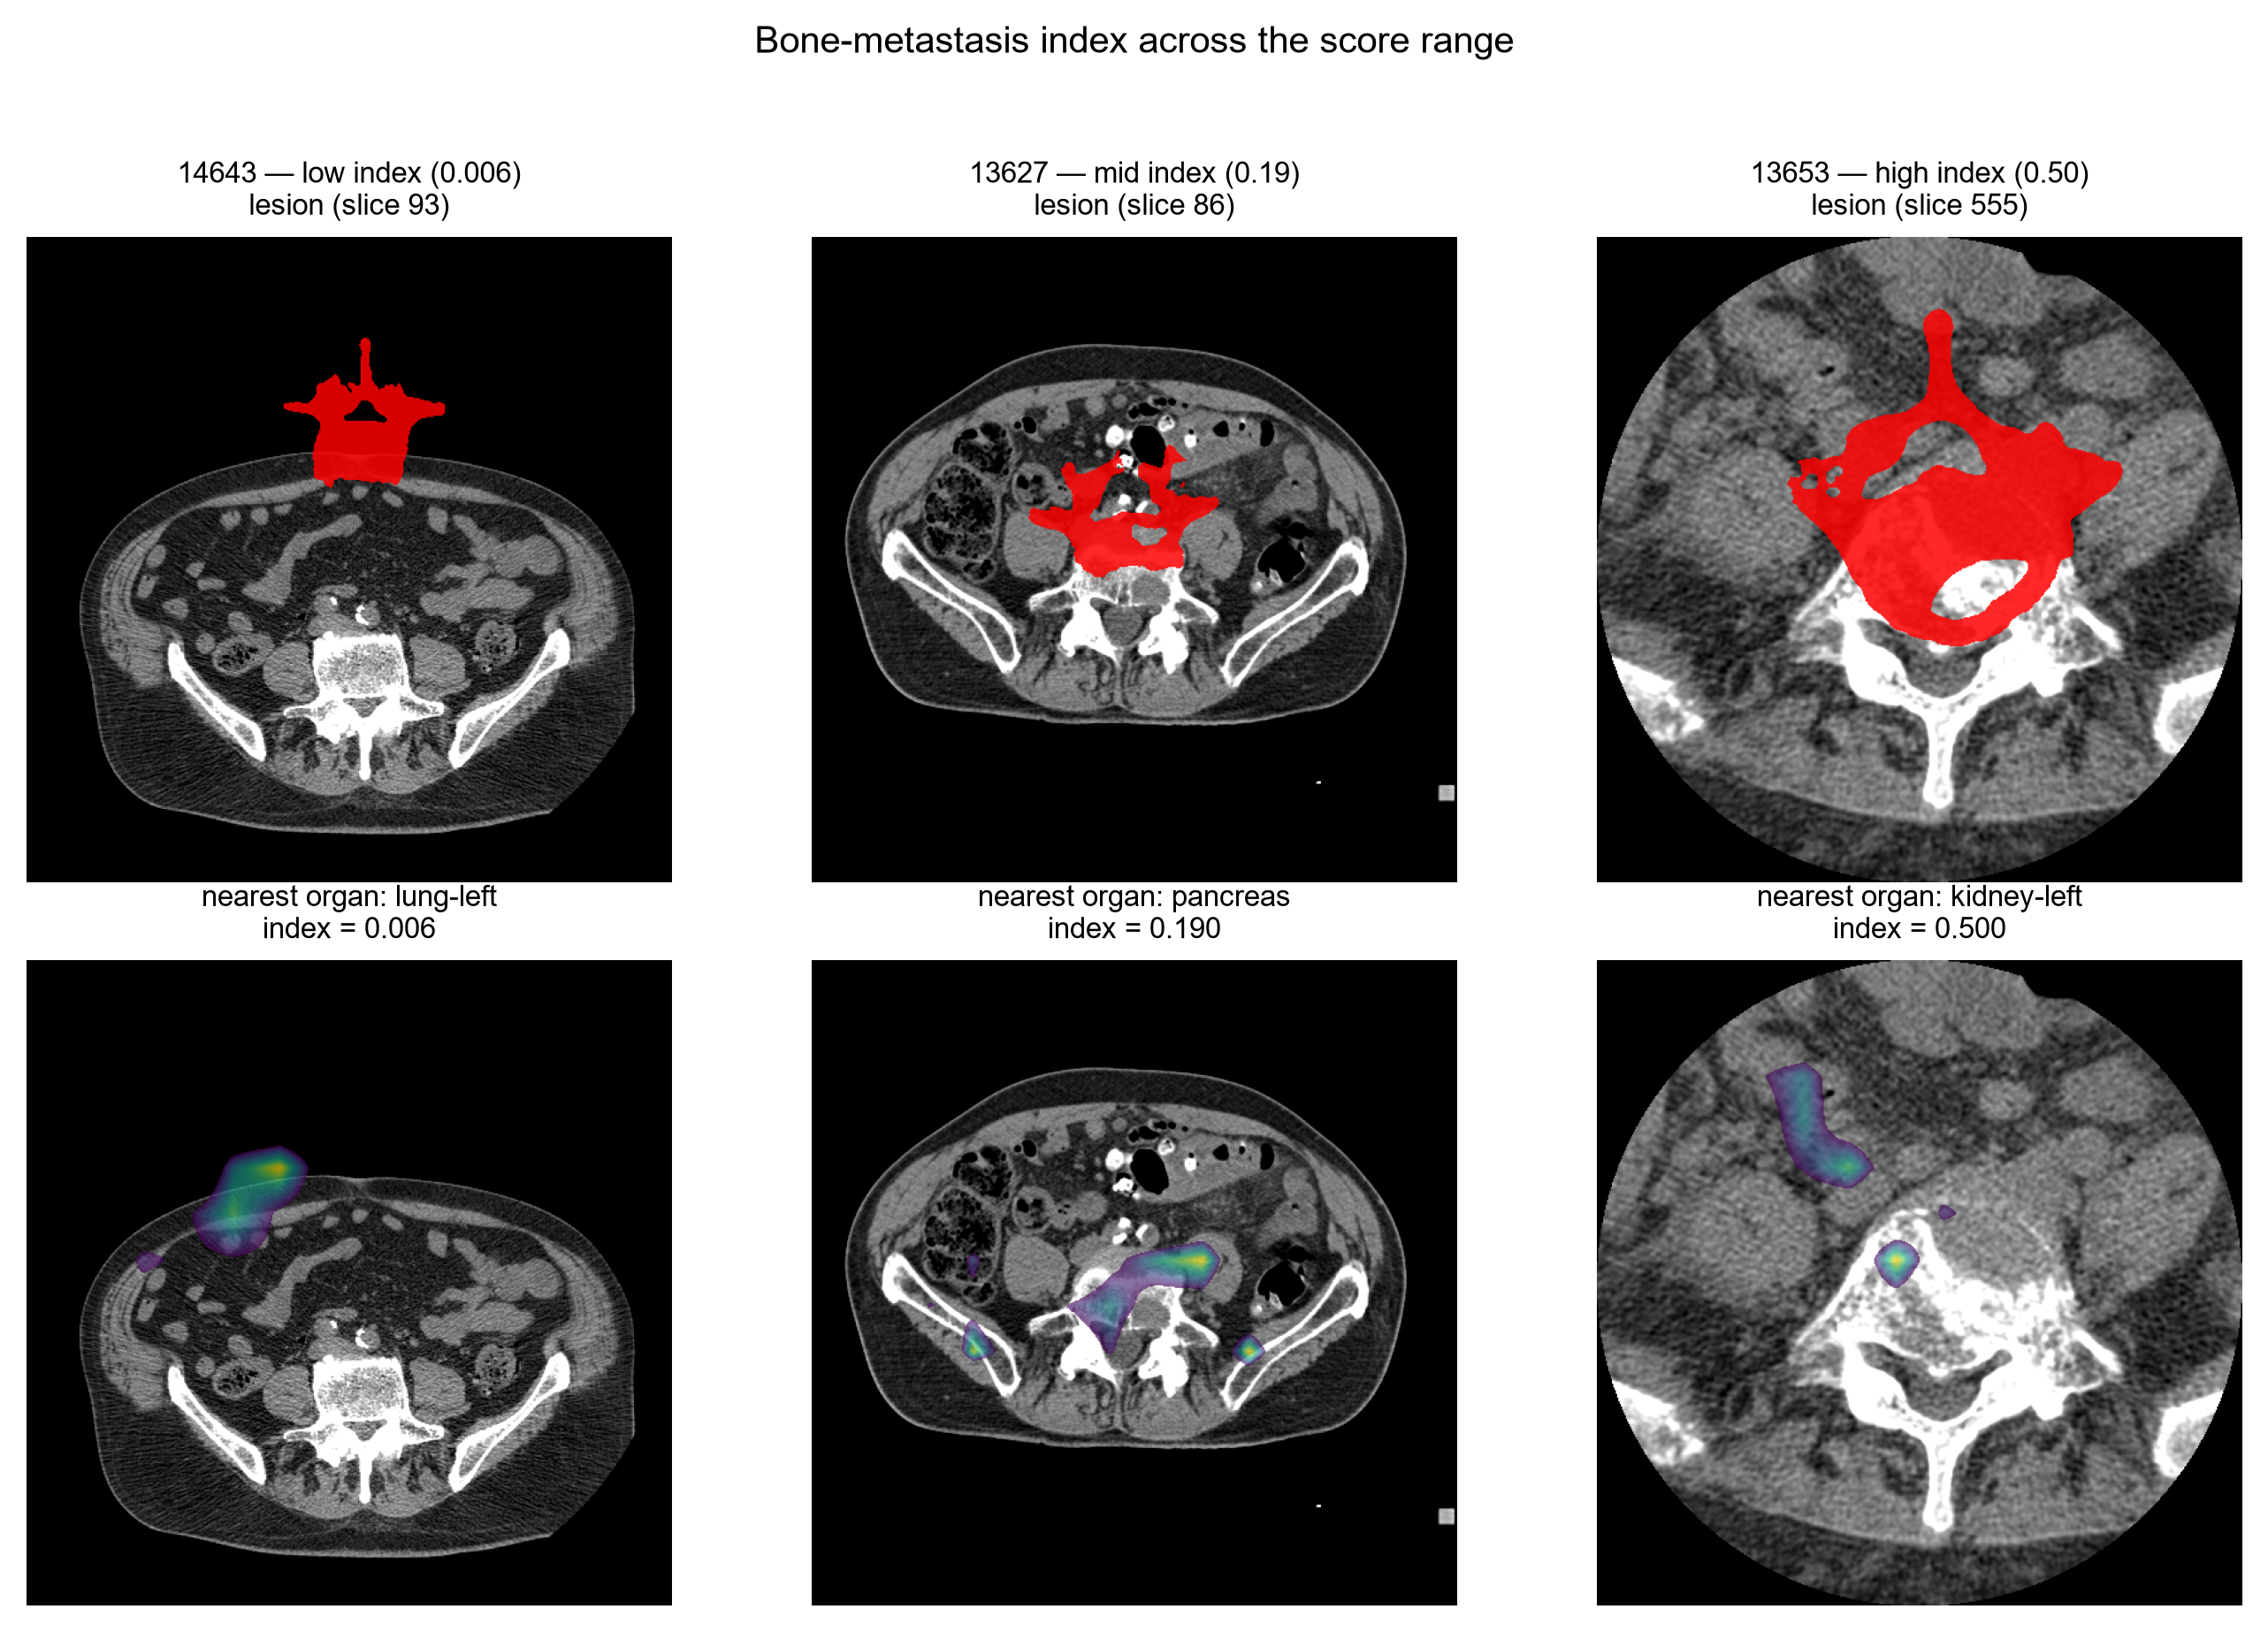
\includegraphics[width=\textwidth]{fig5_spine_lesion_overlays.png}
\caption{Three patients spanning the index range: 14643 (0.006), 13627 (0.190),
13653 (0.500, the cohort maximum). Top: ground-truth lesion mask on the
peak-tumor slice. Bottom: similarity map for the highest-scoring organ against
that lesion. The progression is the point: at low index the nearest-organ map
sits well away from the lesion, and at high index it is effectively touching it.
The low-index panel names \org{lung-left} as nearest organ at a pelvic slice.
This is a phantom detection of the kind we characterize in
\S\ref{sec:results:lesion}, and we retain rather than hide it because the low
index value correctly reflects that nothing real is near this lesion.}
\label{fig:lesionoverlays}
\end{figure}

\subsection{Per-lesion validation}
\label{sec:results:lesion}

Per-patient validation caps out at 20 evaluation points, namely patients with
exactly one involved vertebral level. Scoring per lesion instead, one point per
labelled vertebra and still one inference pass per patient, raises this to 180
lesions across 46 patients, of which 178 are rankable.

Our metric is the rank of the nearest anatomically expected organ in the model's
distance-ordered list, so chance depends on how many organs are expected at that
level and we compute it as the corresponding order statistic
$(n_{\text{organs}}+1)/(k+1)$ for $k$ expected organs.

\textbf{Mean rank is 1.78} (95\% CI $[1.56, 2.03]$), against a chance mean rank
of 2.91, with permutation $p < 0.0001$, and chance lies outside the confidence
interval. Top-1 accuracy is 0.622 and top-3 is 0.894. All our uncertainty
estimates resample \emph{patients}, never lesions: 180 lesions from 46 patients
are not 180 independent trials, since lesions within a patient share a scan and
a set of organ maps. Treating them as independent would inflate significance by
roughly the square root of the average lesions-per-patient, about $2\times$
here, which is larger than any effect our method changes produced.

\paragraph{The result is structured by level, not uniform.}
We consider Figure~\ref{fig:perlevel} the more informative view. Every thoracic
level T1--T11 beats chance, with T8 and T9 perfect (mean rank 1.00). L3 and L4
beat chance clearly. Four levels (T12, L1, L2 and L5) sit at or below chance.
The failure is therefore localized to the thoracolumbar junction rather than
distributed across the method.

\paragraph{A ground-truth error, found and corrected from the literature.}
Our expected-organ table originally dropped the lungs abruptly after T10.
Anatomical sources place the caudal extent of the costophrenic recess at T11 or
below, never above it, so the table was wrong and we corrected it on that basis.
We decided the correction from the literature \emph{before} applying it, and we
did not select it by checking which variant improved the metric. It moved mean
rank $1.94 \to 1.78$ and anatomically impossible top-1 detections $38 \to 34$.
Appendix~\ref{app:anatomy} reproduces the reasoning and sources.

It also moved T11 from below chance to above it, for two compounding reasons:
the answer key at that level became correct, and the expected set became larger,
which lowers chance there. Our earlier descriptions of this result named
``T11--L2'' as the failure band. The correct band after the fix is T12--L2 plus
L5. We now derive band membership in the figure from each level's own
observed-versus-chance comparison rather than from a hardcoded list of level
names, so this particular staleness cannot recur.

\paragraph{Residual failures.}
34 of 180 lesions top-rank an anatomically impossible organ, concentrated in
bladder and femur phantoms. Counting top-rank wins by class makes the
concentration explicit: \org{bladder} takes top rank on 29 lesions, 21 of them
anatomically wrong and 8 correct, while \org{femur-left} and \org{femur-right}
take top rank on 14 lesions of which \emph{none} are correct. The femur classes
never rank first at a level where a femur is expected.
Figure~\ref{fig:qualitative} contrasts a correct detection with one of these
phantoms and shows what the model is actually responding to.

\begin{figure}[t]
\centering
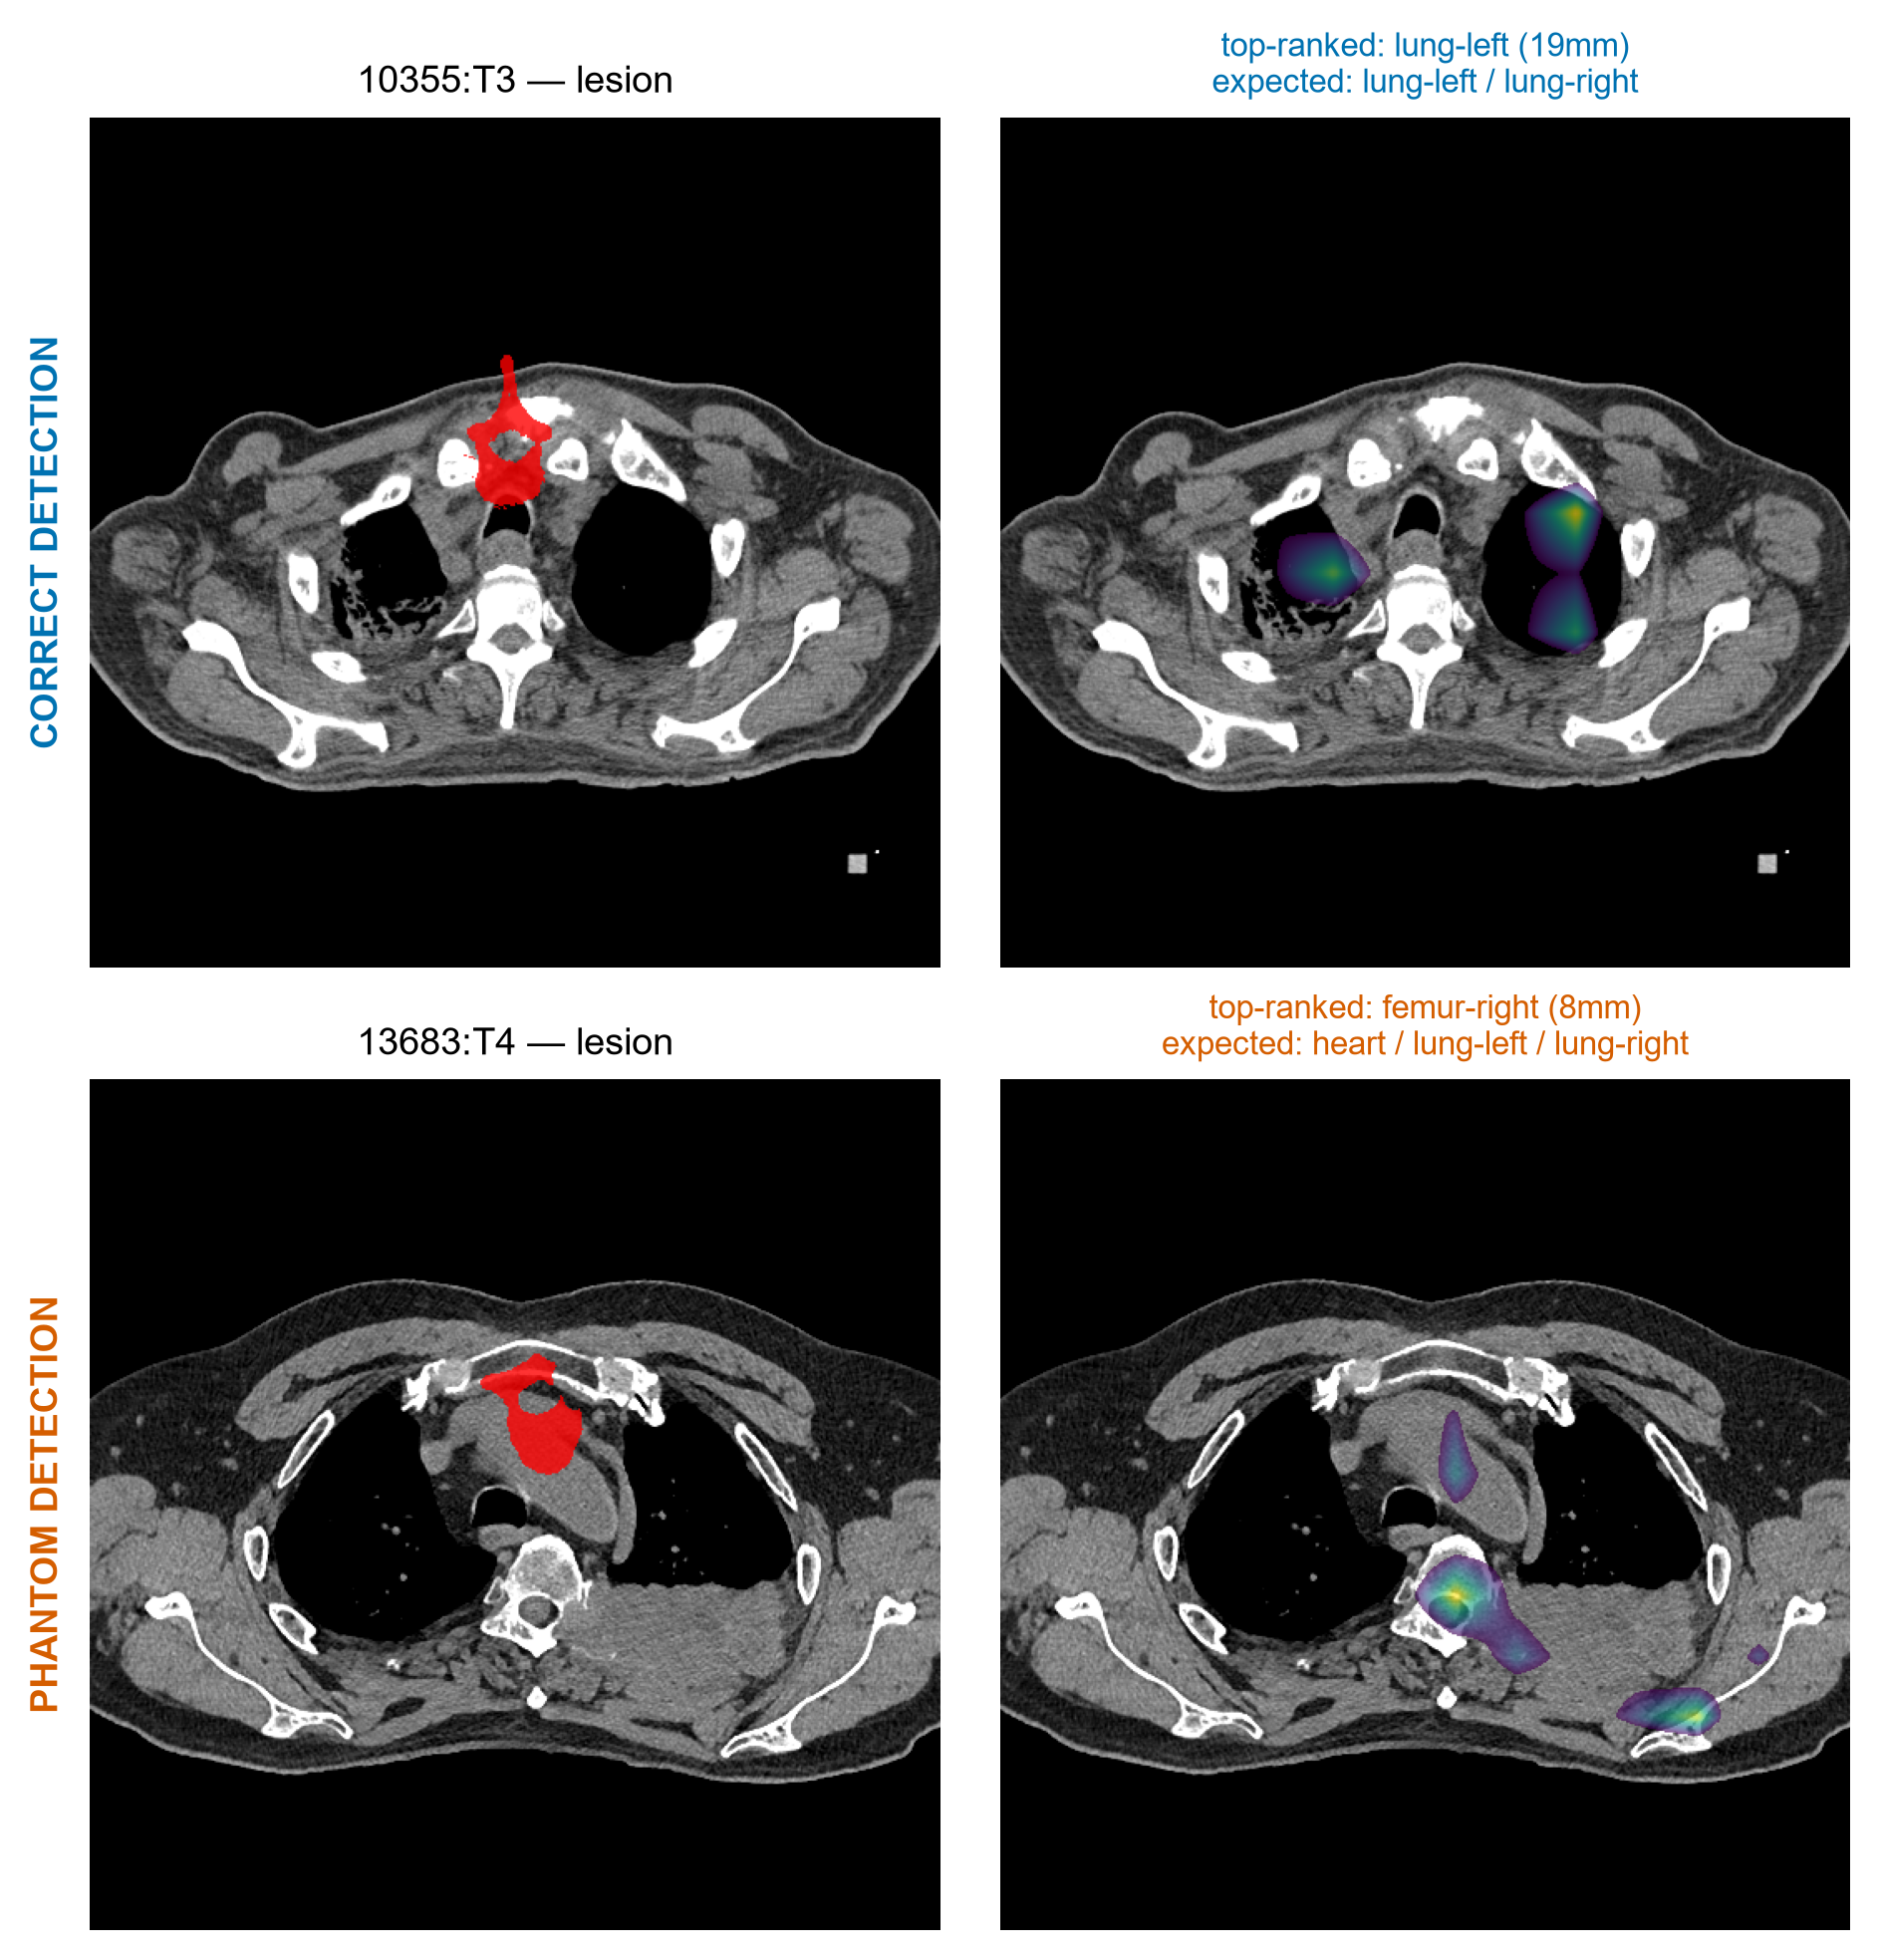
\includegraphics[width=0.58\textwidth]{fig3_qualitative.png}
\caption{Correct localization versus a phantom. Left: CT at the lesion's peak
axial position with the ground-truth mask (red). Right: raw patch-text
similarity for the top-ranked organ at that slice, thresholded to the top 2\% of
that slice's own distribution. \textbf{Top:} case 10355, T3, with
\org{lung-left} correctly ranked first at 19\,mm. \textbf{Bottom:} case 13683,
T4, with \org{femur-right} incorrectly ranked first at 8\,mm, ahead of heart,
\org{lung-left} and \org{lung-right}. The highlighted patches sit on rib
cross-sections at three separate points around the chest wall, not on any
structure resembling a femur shaft.}
\label{fig:qualitative}
\end{figure}

\subsection{Two negative results on the phantom failure mode}
\label{sec:results:negatives}

We tested two hypotheses for the phantom pattern. We fixed both configurations
in advance and report them as run, without retuning.

\paragraph{Field of view: rejected.}
The simplest explanation is that phantom patients' scans do not extend far
enough caudally to contain the true organ, so a wrong organ wins by default. Our
header-only scan-coverage measurement rejects this: phantom patients have
\emph{more} caudal coverage than clean ones (median 122\,mm vs.\ 88.5\,mm below
the last segmented vertebra), and 9 of 12 reach L5.

\paragraph{Missing vocabulary classes.}
Our text-encoder-only diagnostic showed that the \org{femur} prompt embeds
almost identically to an undefined \org{humerus} prompt, more closely than to
any of femur's own defined classmates, and that the \org{bladder} prompt's
nearest neighbour is an undefined \org{aorta} prompt. This motivated us to add
rib, humerus and aorta as negative prompts.

\paragraph{Calibration variants.}
Table~\ref{tab:variants} reports both variants. We adopt neither.

\begin{table}[t]
\centering
\small
\caption{Calibration variants, each a single pre-registered run.
\textbf{Both variants predate our T11/T12 ground-truth correction} and are
scored against the stricter pre-fix expected-organ table, so their comparator is
the pre-fix baseline row (mean rank 1.94), not the current headline 1.78. That
difference is the answer key changing, not the method. Chance moves with the key
too: 3.01 pre-fix, 2.91 post-fix.}
\label{tab:variants}
\begin{tabular}{@{}llrrrrrr@{}}
\toprule
Variant & Key & \makecell{Mean\\rank} & Top-1 & Top-3 & Ranked & \makecell{Imposs.\\top-1} & \makecell{Pair\\splits} \\
\midrule
\textbf{Baseline, current} & post-fix & \textbf{1.78} & 0.62 & 0.89 & 178/180 & 34/180 & 34/540 \\
Baseline, pre-fix \emph{(comparator)} & pre-fix & 1.94 & 0.59 & 0.86 & 178/180 & 38/180 & 34/540 \\
$+$ rib/humerus/aorta negatives & pre-fix & 2.04 & 0.53 & 0.82 & 171/180 & 37/180 & 58/540 \\
Z-score floor ($\mu + 2\sigma$) & pre-fix & 1.82 & 0.50 & 0.83 & 164/180 & 79/180 & 0/540 \\
\bottomrule
\end{tabular}
\end{table}

Global hard negatives traded one confusion for another. Femur pair-splitting
improved sharply ($31 \to 4$), but a \emph{new} lung pair-splitting problem
appeared ($0 \to 46$ of 540), and top-1 and top-3 both fell. The mechanism is
specific: we subtracted the rib negative from \emph{every} organ's score rather
than only from femur's, so it bled into the lungs' own scoring at the rib-lung
boundary, where lung tissue legitimately abuts rib.

The z-score floor moved mean rank in the right direction ($1.94 \to 1.82$) and
eliminated bilateral pair splitting entirely ($34 \to 0$ of 540), but more than
doubled anatomically impossible detections ($38 \to 79$). Nearly every wrong
detection wins at 0--1\,mm, which is consistent with the floor being too
permissive: instead of correctly vanishing where an organ is absent, most organs
retain a sliver of territory almost everywhere, and a sliver is enough to win a
proximity contest.

One methodological caution applies to reading Table~\ref{tab:variants}. Both
variants leave more lesions unrankable than the baseline (171 and 164 vs.\ 178),
so their mean ranks average over a smaller and easier subset, which flatters
that column. Top-1 and top-3 are computed over all 180 and are the cleaner
comparison. Both variants fall on those, which points the same way as the
impossible-detection counts.
